\section{Aplicación}
\subsubsection{Introducción}

En el apartado de aplicación se presenta el modelamiento de la aplicación dentro de la organización. La arquitectura de aplicación analiza si cada uno de los sistemas satisface ciertos criterios de calidad respecto a los procesos de negocio. Concluyendo de esta manera la importancia de la aplicación para la organización.

\newpage

\subsubsection{Punto de Vista de Comportamiento de aplicación}

El punto de vista de comportamiento de aplicación se presentan los componentes involucrados en la organización.

%%grafo

\begin{figure}[th!]
	\centering
	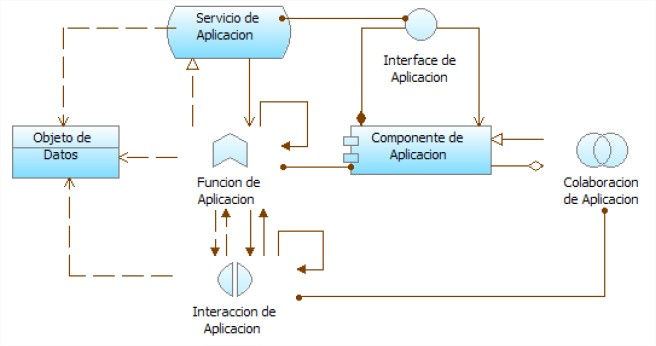
\includegraphics[width=13cm,height=6cm]{arquitectura/aplicacion/imgs/comportamiento-e}
	\caption{Modelo de Comportamiento de aplicación}{\scriptsize \textbf{Fuente:} Archimate 2.0 \cite{WEB7}}
\end{figure}

\subsubsection{Caso}

En la organización se definen los siguientes componentes que interactuan en la aplicación de desarrollo.

%%grafo
\begin{figure}[th!]
	\centering
	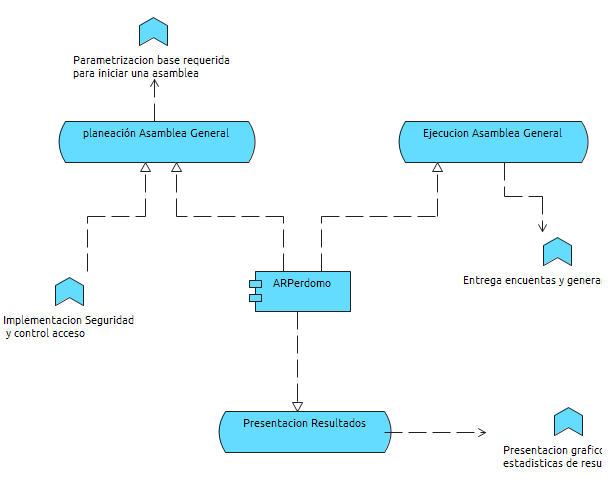
\includegraphics[width=13cm,height=7cm]{arquitectura/aplicacion/imgs/comportamiento}
	\caption{Caso de Comportamiento de aplicación}{\scriptsize \textbf{Fuente:} Imagen propia}
\end{figure}

\subsubsection{Punto de Vista de Cooperación de aplicación}

El punto de vista de cooperación de aplicación se presentan los componentes involucrados en la aplicación desarrollada en la organización.

%%grafo

\begin{figure}[th!]
	\centering
	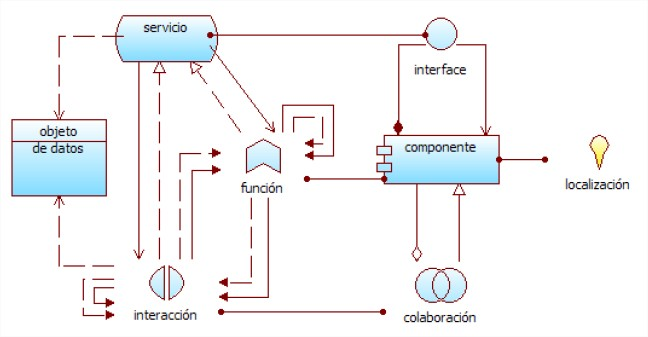
\includegraphics[width=13cm,height=6cm]{arquitectura/aplicacion/imgs/cooperacion-e}
	\caption{Modelo de Cooperación de aplicación}{\scriptsize \textbf{Fuente:} Archimate 2.0 \cite{WEB7}}
\end{figure}

\subsubsection{Caso}

En la organización se definen los siguientes componentes que interactuan en la aplicación de desarrollo para beneficio de la organización.

%%grafo
\begin{figure}[th!]
	\centering
	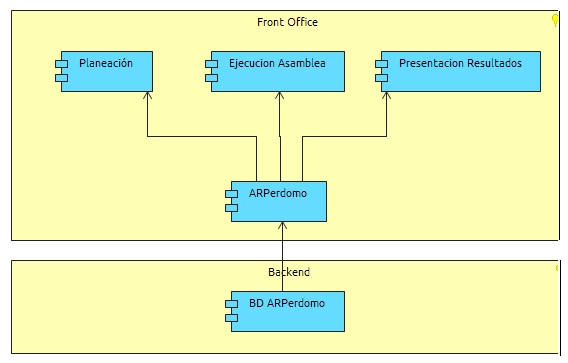
\includegraphics[width=13cm,height=6cm]{arquitectura/aplicacion/imgs/cooperacion}
	\caption{Caso de Cooperación de aplicación}{\scriptsize \textbf{Fuente:} Imagen propia}
\end{figure}


\subsubsection{Punto de Vista de Estructura de aplicación}

El punto de vista de estructura de aplicación se presentan la comunicación de los diferentes componentes de aplicación.

%%grafo

\begin{figure}[th!]
	\centering
	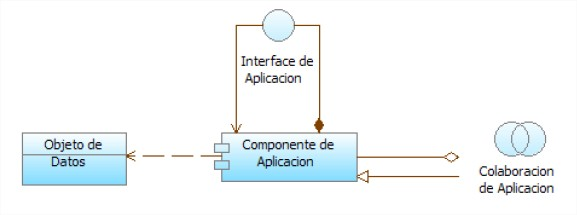
\includegraphics[width=13cm,height=6cm]{arquitectura/aplicacion/imgs/estructura-e}
	\caption{Modelo de Estructura de aplicación}{\scriptsize \textbf{Fuente:} Archimate 2.0 \cite{WEB7}}
\end{figure}

\subsubsection{Caso}

En la organización se definen los siguientes componentes su comunicación e interacción con la aplicación qiue afecta directamente a la organización.

%%grafo
\begin{figure}[th!]
	\centering
	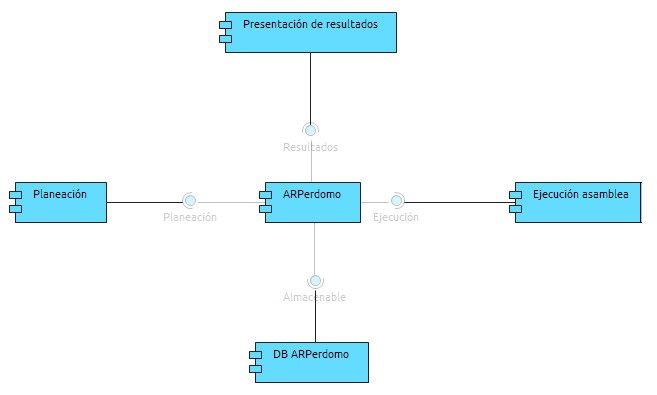
\includegraphics[width=13cm,height=7cm]{arquitectura/aplicacion/imgs/estructura}
	\caption{Caso de Estructura de aplicación}{\scriptsize \textbf{Fuente:} Imagen propia}
\end{figure}


\subsubsection{Punto de Vista de Uso de aplicación}

El punto de vista de uso de aplicación se presentan los componentes con uso dentro de la organización.

%%grafo

\begin{figure}[th!]
	\centering
	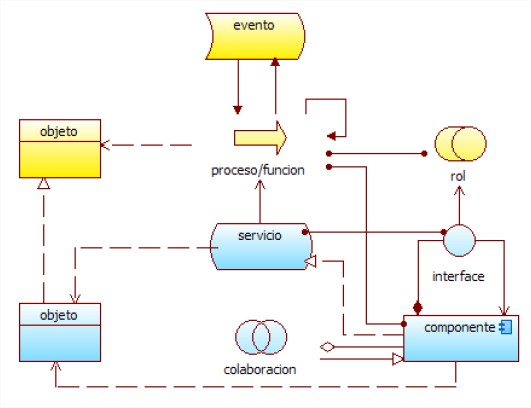
\includegraphics[width=13cm,height=6cm]{arquitectura/aplicacion/imgs/uso-e}
	\caption{Modelo de Uso de aplicación}{\scriptsize \textbf{Fuente:} Archimate 2.0 \cite{WEB7}}
\end{figure}

\subsubsection{Caso}

En la organización se definen los siguientes usos que se contemplan para la aplicación de desarrollo para la empresa.

%%grafo
\begin{figure}[th!]
	\centering
	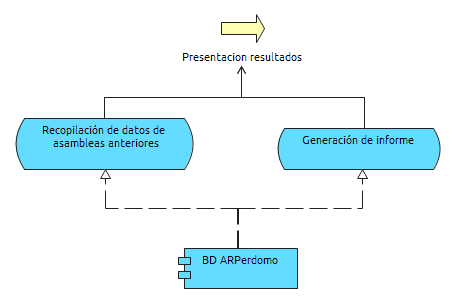
\includegraphics[width=13cm,height=7cm]{arquitectura/aplicacion/imgs/uso}
	\caption{Caso de Uso de aplicación}{\scriptsize \textbf{Fuente:} Imagen propia}
\end{figure}
\newpage